\section{Gammapy package}
\label{sec:package}

The \gammapy package is structured into multiple sub-packages
which mostly follow the stages in the data reduction workflow.


\subsection{Overview}
\begin{figure*}[t]
\centering
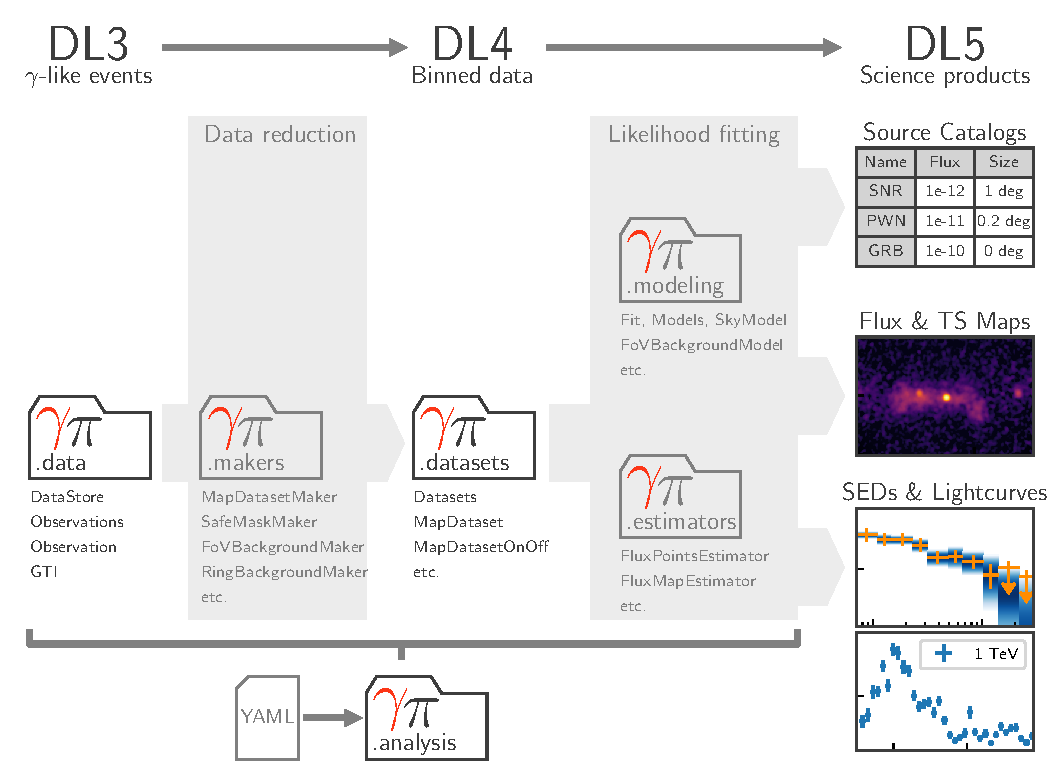
\includegraphics[width=1.\textwidth]{static/data-flow-gammapy}
\caption{
Gammapy sub-package structure and data analysis workflow.
}
\label{fig:workflow}
\end{figure*}


\subsection{gammapy.data}
The \verb|gammapy.data| sub-package provides access to
DL3 level data and observation handling.


\begin{figure}

\import{snippets/generated/}{gp_data}

\caption{Using gammapy.data to access DL3 level data with a DataStore}
\label{fig*:minted}
\end{figure}



\subsection{gammapy.makers}
\todo{Regis Terrier}
Data reduction

\begin{lstlisting}

from gammapy.makers import MapDatasetMaker

maker = MapDatasetMaker()
dataset = maker.run(dataset, observation)

\caption{Using gammapy.data to access DL3 level data}
\label{codeexample:maker}
\end{lstlisting}


\subsection{gammapy.datasets}
\todo{Atreyee Sinha}
DL4 level data


\begin{lstlisting}

from astropy.coordinates import SkyCoord
from gammapy.maps import WcsGeom
from gammapy.datasets import MapDataset

skydir = SkyCoord("0d", "0d")
geom = WcsGeom.create(
	skydir=skydir, width="5 deg", binsz="0.2 deg"
)

dataset = MapDataset.create(
	geom=geom, name="my-dataset"
)


\caption{Using gammapy.data to access DL3 level data with a DataStore}
\label{codeexample:data}
\end{lstlisting}



\subsection{gammapy.modeling}
\todo{Quentin Remy}
Models and fitting

\begin{lstlisting}

from gammapy.modeling.models import (
	SkyModel,
	PowerLawSpectralModel,
	PointSpatialModel
)

pwl = PowerLawSpectralModel()
point = PointSpatialModel()

model = SkyModel(
	spectral_model=pwl,
	spatial_model=point
	name="my-model"
)
\caption{Using gammapy.data to access DL3 level data}
\label{codeexample:maker}
\end{lstlisting}


\subsection{gammapy.estimators}
\todo{Axel Donath}
Estimators

\subsection{gammapy.visualisation}
Plotters etc.

\subsection{gammapy.analysis}
\todo{Jose Enrique writes this...}
High level analysis API

\subsection{gammapy.astro}
Dark matter models, source population modelling

\subsection{gammapy.data}
\todo{Cosimo Nigro}

\subsection{gammapy.catalog}
Gamma-ray catalog access

\begin{lstlisting}

from gammapy.catalog import SOURCE_CATALOGS

\caption{Using gammapy.data to access DL3 level data with a DataStore}
\label{codeexample:data}
\end{lstlisting}


\subsection{gammapy.maps}
\todo{Laura Olivera-Nieto}
The \verb|gammapy.maps| sub-package provides classes for representing pixelized
data structures with at least two spatial dimensions representing a set of
coordinates or a region on a sphere. In addition it allows to handle and arbitray
number of non-spatial data axes, such as time or energy.

It provides a uniform API for WCS, HEALPix and region based data structures.

\begin{lstlisting}

from gammapy.maps import Map
from astropy.coordinates import SkyCoord

skydir = SkyCoord("0d", "5d", frame="galactic")

# Create a WCS Map
m_wcs = Map.create(
	binsz=0.1, map_type='wcs', skydir=skydir, width=10.0
)

# Create a HPX Map
m_hpx = Map.create(
	binsz=0.1, map_type='hpx', skydir=skydir, width=10.0
)

\caption{Using gammapy.data to access DL3 level data with a DataStore}
\label{codeexample:data}
\end{lstlisting}


\subsection{gammapy.irf}
\todo{Fabio Pintore}
IRF classes

\subsection{gammapy.stats}
\todo{Regis Terrier}
Statistics methods


\subsection{gammapy.utils}
Utility functions...


Outline:
* List typical analysis use cases
* Can use from Python and Jupyter -> show Figure with Jupyter notebook here.
* Gammapy code structure
* How Numpy and Astropy is used


Figures:
* Add a Figure showing dataflow in a typical application
DL3 at the top, spectrum, map, lightcurve, fit results at the bottom.
Mention major classes in between (DataStore, EventList, Map, MapMaker, MapFit, …)
* Probably not: Figure showing sub-packages and how they relate (gammapy.data and gammapy.irf at the base, then gammapy.maps, etc.
* The code example Figure how to make a counts map, to explain how the package works.
